\documentclass[submit]{harvardml}

\course{CS181-S22}
\assignment{Assignment \#1}
\duedate{7:59pm ET, February 4, 2022} 

\usepackage[OT1]{fontenc}
\usepackage[colorlinks,citecolor=blue,urlcolor=blue]{hyperref}
\usepackage[pdftex]{graphicx}
\usepackage{graphicx}
\usepackage{caption}
\usepackage{fullpage}
\usepackage{soul}
\usepackage{amsmath}
\usepackage{amssymb}
\usepackage{color}
\usepackage{todonotes}
\usepackage{listings}
\usepackage{common}
\usepackage{framed}

\usepackage[mmddyyyy,hhmmss]{datetime}

\definecolor{verbgray}{gray}{0.9}

\lstnewenvironment{csv}{
  \lstset{backgroundcolor=\color{verbgray},
  frame=single,
  framerule=0pt,
  basicstyle=\ttfamily,
  columns=fullflexible}}{}
 

\begin{document}
\begin{center}
{\Large Homework 1: Regression}\\
\end{center}

\subsection*{Introduction}
This homework is on different forms of linear regression and focuses
on loss functions, optimizers, and regularization. Linear regression
will be one of the few models that we see that has an analytical
solution.  These problems focus on deriving these solutions and
exploring their properties.

If you find that you are having trouble with the first couple
problems, we recommend going over the fundamentals of linear algebra
and matrix calculus (see links on website).  The relevant parts of the
\href{https://github.com/harvard-ml-courses/cs181-textbook/blob/master/Textbook.pdf}{cs181-textbook notes are Sections 2.1 - 2.7}.  We strongly recommend
reading the textbook before beginning the homework.

    We also encourage you to first read the \href{http://users.isr.ist.utl.pt/~wurmd/Livros/school/Bishop\%20-\%20Pattern\%20Recognition\%20And\%20Machine\%20Learning\%20-\%20Springer\%20\%202006.pdf}{Bishop textbook}, particularly:
Section 2.3 (Properties of Gaussian Distributions), Section 3.1
(Linear Basis Regression), and Section 3.3 (Bayesian Linear
Regression). (Note that our notation is slightly different but the
underlying mathematics remains the same!).

\textbf{Please type your solutions after the corresponding problems using this
\LaTeX\ template, and start each problem on a new page.} You may find
the following introductory resources on \LaTeX\ useful: 
\href{http://www.mjdenny.com/workshops/LaTeX_Intro.pdf}{\LaTeX\ Basics} 
and \href{https://www.overleaf.com/learn/latex/Free_online_introduction_to_LaTeX_(part_1)}{\LaTeX\ tutorial with exercises in Overleaf}

Homeworks will be submitted through Gradescope. You will be added to
the course Gradescope once you join the course Canvas page. If you
haven't received an invitation, contact the course staff through Ed.

\textbf{Please submit the writeup PDF to the Gradescope assignment
  `HW1'.} Remember to assign pages for each question.

\textbf{Please submit your \LaTeX file and code files to the
  Gradescope assignment `HW1 - Supplemental'.} Your files should be
named in the same way as we provide them in the repository,
e.g. \texttt{T1\_P1.py}, etc.


%%%%%%%%%%%%%%%%%%%%%%%%%%%%%%%%%%%%%%%%%%%%%
% Problem 1
%%%%%%%%%%%%%%%%%%%%%%%%%%%%%%%%%%%%%%%%%%%%%

\begin{problem}[Optimizing a Kernel, 15pts]

Kernel-based regression techniques are similar to nearest-neighbor
regressors: rather than fit a parametric model, they predict values
for new data points by interpolating values from existing points in
the training set.  In this problem, we will consider a kernel-based
regressor of the form:
\begin{equation*}
  f(x^*) = \sum_{n} K(x_n,x^*) y_n 
\end{equation*}
where $(x_n,y_n)$ are the training data points, and $K(x,x')$ is a
kernel function that defines the similarity between two inputs $x$ and
$x'$. Assume that each $x_i$ is represented as a column vector, i.e. a
$D$ by 1 vector where $D$ is the number of features for each data
point. A popular choice of kernel is a function that decays as the
distance between the two points increases, such as
\begin{equation*}
  K(x,x') = \exp\left(\frac{-||x-x'||^2_2}{\tau}\right) = \exp\left(\frac{-(x-x')^T (x-x')}{\tau} \right) 
\end{equation*}
where $\tau$ represents the square of the lengthscale (a scalar value).  In this
problem, we will consider optimizing what that (squared) lengthscale
should be.

\begin{enumerate}

\item Let $\{(x_n,y_n)\}_{n=1}^N$ be our training data set.  Suppose
  we are interested in minimizing the residual sum of squares.  Write
  down this loss over the training data $\mcL(W)$ as a function of $\tau$.

  Important: When computing the prediction $f(x_i)$ for a point $x_i$
  in the training set, carefully consider for which points $x'$ you should be including
  the term $K(x_i,x')$ in the sum.

\item Take the derivative of the loss function with respect to $\tau$.
\end{enumerate}

\end{problem}

\newpage

\begin{framed}
\noindent\textbf{Problem 1} (cont.)\\

\begin{enumerate}
\setcounter{enumi}{2}
\item Consider the following data set:
\begin{csv}
  x , y
  0 , 0
  1 , 0.5
  2 , 1
  3 , 2
  4 , 1
  6 , 1.5
  8 , 0.5 
\end{csv}
And the following lengthscales: $\tau=.01$, $\tau=2$, and $\tau=100$.

Write some Python code to compute the loss with respect to each kernel
for the dataset provided above. Which lengthscale does best?  
For this problem, you can use our staff \textbf{script to compare your
  code to a set of staff-written test cases.} This requires, however,
that you use the structure of the starter code provided in
\texttt{T1\_P1.py}. More specific instructions can be found at the top
of the file \texttt{T1\_P1\_Testcases.py}. You may run the test cases
in the command-line using \texttt{python T1\_P1\_TestCases.py}.
\textbf{Note that our set of test cases is not comprehensive: just
  because you pass does not mean your solution is correct! We strongly
  encourage you to write your own test cases and read more about ours
  in the comments of the Python script.}
  
\item Plot the function $(x^*, f(x^*))$ for each of the
  lengthscales above.  You will plot $x^*$ on the x-axis and the
  prediction $f(x^*)$ on the y-axis.  For the test inputs $x^*$, you
  should use an even grid of spacing of $0.1$ between $x^* = 0$ and
  $x^* = 12$.  (Note: it is possible that a test input $x^*$ lands
  right on top of one of the training inputs above.  You can still use
  the formula!) 

  Initial impressions: Briefly describe what happens in each of the
  three cases.  Is what you see consistent with the which lengthscale
  appeared to be numerically best above?  Describe why or why not.

\item Bonus: Code up a gradient descent to optimize the kernel for the
  data set above.
  Start your gradient descent from $\tau=2$. Report on what you
  find.\\\\

  Note: Gradient descent is discussed in Section 3.4 of the
  cs181-textbook notes and Section 5.2.4 of Bishop, and will be
  covered later in the course!

\end{enumerate}
  
\end{framed}  
\newpage
\noindent \textbf{Solution 1.1:}\\ \\
\[L(\tau) = \sum_{n=1}^{N} \left( y_n - \sum_{i=1, i\neq n}^N \exp\left(\frac{-(x_i-x_n)^T (x_i-x_n)}{\tau} \right)y_i \right)^2 \] \\ \\
\textbf{Solution 1.2:}\\ \\
\begin{align*}
\frac{d}{d\tau}\left(L(\tau)\right) &= \frac{d}{d\tau}\left(\sum_{n=1}^{N} \left( y_n - \sum_{i=1, i\neq n}^N \exp\left(\frac{-(x_i-x_n)^T (x_i-x_n)}{\tau} \right)y_i \right)^2\right)\\
&= \sum_{n=1}^{N}  \left[2\left( y_n - \sum_{i=1, i\neq n}^N \exp\left(\frac{-(x_i-x_n)^T (x_i-x_n)}{\tau} \right)y_i \right) \\
&\cdot \left\left(\sum_{i=1, i\neq n}^N \exp\left(\frac{-(x_i-x_n)^T (x_i-x_n)}{\tau} \right) \left(\frac{(x_i-x_n)^T (x_i-x_n)}{\tau^2} \right)y_i \right) \right]
\end{align*} \\ \\
\textbf{Solution 1.3:}\\ \\
The lengthscale $\tau = 2$ performs best, with loss of $\approx 3.31$. \\ \\ \\
\textbf{Solution 1.4:}

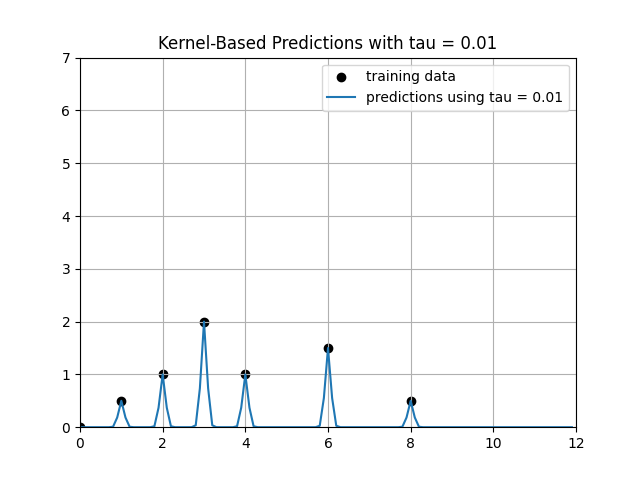
\includegraphics[scale=0.75]{tau0.01.png} \\

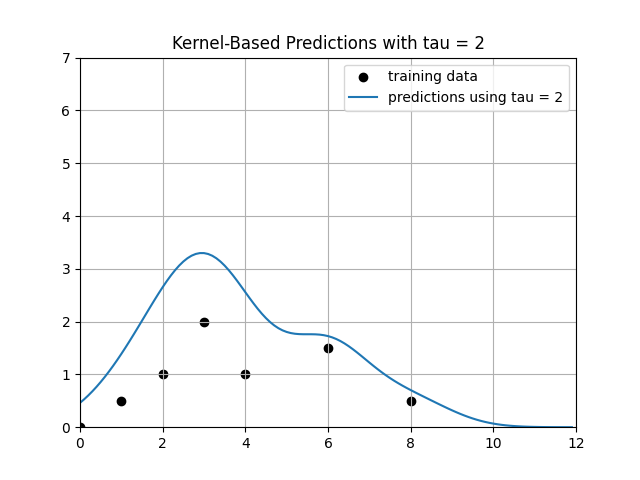
\includegraphics[scale=0.75]{tau2.png} \\

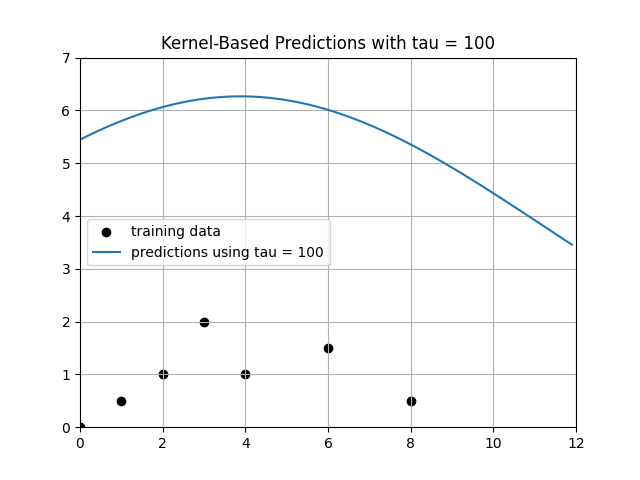
\includegraphics[scale=0.75]{tau100.png} \\
\noin In the first graph, where $\tau = 0.01$, the kernel function decays at a very sharp rate, causing the regressor to predict extremely low values (almost 0) for inputs which are not proximal to points within the training data. Because of this sharp decay, the regressor also generates extremely accurate predictions for inputs which coincide with a point the training data as there is no additional noise generated because of the sharp decay. As such, the graph of $f(x^*)$ for $\tau = 0.01$ appears to jump up to accurately predict inputs within the training dataset and drop to extremely low values for all other intermediate inputs between points in the training data. \\ \\
\noin In the second graph, were $\tau = 2$, the kernel function seems to decay at a reasonable rate, allowing the regressor to predict intermediate input between training data points with relative accuracy. Compared to the first graph, the regressor does not predict inputs within the training data to the same degree of accuracy because the more gradual decay of the kernel functions results in some noise leading a slightly larger prediction. However, overall, the graph of $f(x^*)$ for $\tau = 2$ appears to follow the general trend of the data points within the training data, while erring on the side of over-prediction. \\ \\
\noin In the third graph, where $\tau = 100$, the kernel function decays at a very slow rate, leading the regressor to generate overly large predictions. As such, the graph of the $f(x^*)$ for $\tau = 100$ displays values that are much larger than the values of the training data set; however, the graph does loosely follow the shape of the data. \\ \\
\noin Overall, these graphs are consistent with the numerical loss calculated above. The graph with lengthscale 2 displays the highest accuracy, which would correspond the lowest amount of loss. While the first graph shows the highest accuracy for inputs in the data set, within our loss function, we omitted a data point when calculating its own prediction, meaning all predictions were very close to 0, and thus causing loss to be  greater. The third lengthscale performed the worst in terms of loss, which corresponds the graph in which it grossly overestimates.
\newpage

%%%%%%%%%%%%%%%%%%%%%%%%%%%%%%%%%%%%%%%%%%%%%
% Problem 2
%%%%%%%%%%%%%%%%%%%%%%%%%%%%%%%%%%%%%%%%%%%%%

\begin{problem}[Kernels and kNN, 10pts]

Now, let us compare the kernel-based approach to an approach based on
nearest-neighbors.  Recall that kNN uses a predictor of the form
  \begin{equation*}
    f(x^*) = \frac{1}{k} \sum_n y_n \mathbb{I}(x_n \texttt{ is one of k-closest to } x^*)
  \end{equation*}

\noindent where $\mathbb{I}$ is an indicator variable. For this problem, you will use the \textbf{same dataset and kernel as in Problem 1}.


For this problem, you can use our staff \textbf{script to compare your code to a set of staff-written test cases.} This requires, however, that you use the structure of the starter code provided in \texttt{T1\_P2.py}. More specific instructions can be found at the top of the file \texttt{T1\_P2\_Testcases.py}. You may run the test cases in the command-line using \texttt{python T1\_P2\_TestCases.py}.
\textbf{Note that our set of test cases is not comprehensive: just because you pass does not mean your solution is correct! We strongly encourage you to write your own test cases and read more about ours in the comments of the Python script.}

\vspace{0.5cm}
\noindent\emph{Make sure to include all required plots in your PDF.}


\begin{enumerate}

\item Implement kNN for $k=\{1, 3, N-1\}$ where N is the size of the dataset, then plot the results for each $k$. To find the distance between points, use the kernel function from Problem 1 with lengthscale $\tau=1$. 

As before, you will plot $x^*$ on the x-axis and the prediction $f(x^*)$ on the y-axis.  For the test inputs $x^*$, you should use an even grid of spacing of $0.1$ between $x^* = 0$ and $x^* = 12$.  (Like in Problem 1, if a test point lies on top of a training input, use the formula without excluding that training input.)
  
  You may choose to use some starter Python code to create your plots
  provided in \verb|T1_P2.py|.  Please \textbf{write your own
    implementation of kNN} for full credit.  Do not use external
  libraries to find nearest neighbors.
  
\item Describe what you see: What is the behavior of the functions in
  these three plots?  How does it compare to the behavior of the
  functions in the three plots from Problem 1?  Are there situations
  in which kNN and kernel-based regression interpolate similarly?
  Extrapolate similarly?  Based on what you see, do you believe there
  exist some values of $k$ and $\tau$ for which the kNN and kernel-based regressors produce the exact same classifier (ie. given \textit{any} point $x$, the two regressors will produce the same prediction $f(x)$)? Explain your answer.
  
\item Why did we not vary $\tau$ for the kNN approach?

\end{enumerate}

\end{problem}


\newpage 
\textbf{Solution 2.1:}\\ \\

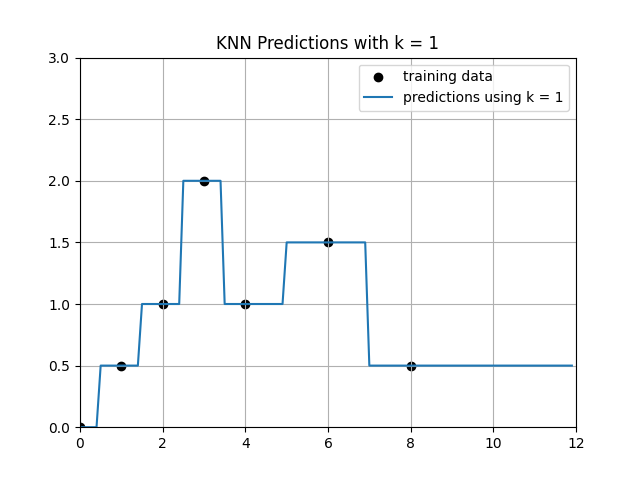
\includegraphics[scale=0.75]{k1.png} \\

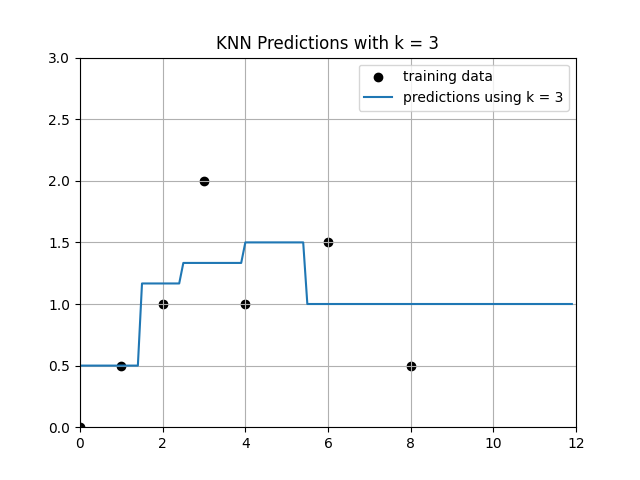
\includegraphics[scale=0.75]{k3.png} \\

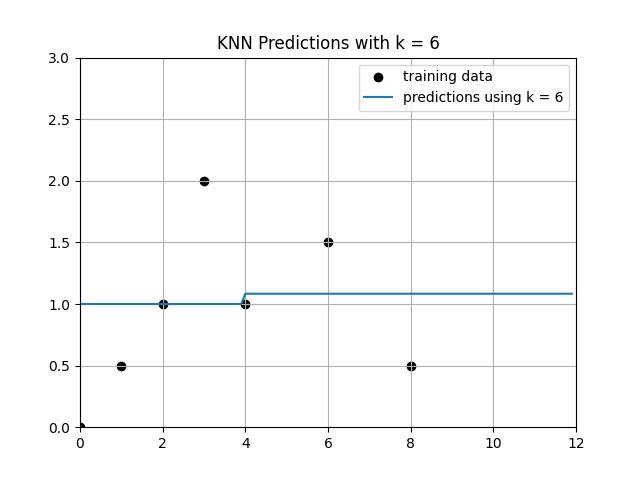
\includegraphics[scale=0.75]{k6.png} \\
\noin \textbf{Solution 2.2:} \\ \\
\noin Looking at the behavior of the functions in these three plots, it appears that lower values of $k$ correspond higher predictive accuracy. This is because for larger values of $k$, it is more likely that points will have the same $k$ nearest neighbors, leading the function to hold constant at an average value within the dataset as we see for the graph where $k=6$. For lower values of $k$, only the most proximal training data points will affect the regressor's prediction for a given input, leading the regressor to more closely mirror the shape of the training data set. Moreover, with lower $k$, different inputs will have different $k$ nearest neighbors, allowing the function to fluctuate rather than converge to a single value. This can be seen in the graph where $k=1$. \\ \\
Compared to the kernel-based regressor, the graph of the kNN approach looks similar to a piecewise step function, for certain range of inputs, the regressor's prediction is held constant at a single output. This is because distinct inputs within a certain range have the same $k$ nearest neighbors and thus, the function will generate the same prediction for all of them. Comparatively, the kernel-based regressor relies on a kernel function which decays exponentially with distance from a given point in the training data. As such, the graphs using this approach look more fluid compared to kNN as predictions are gradually incremented or decremented for inputs. \\ \\
In terms of interpolation, the kNN approach appears to have highly accurate interpolation for low values of $k$, as seen in the graph where $k=1$, and kernel-based regressor's appear to have highly accurate interpolation for low values of $\tau$, as seen in the graph where $\tau = 0.01$. \\ \\
For extrapolation, the lower values of $k$ still appear to do better in the kNN approach, as seen when comparing $k=1$ and $k=6$. The graph of $k=6$ largely remains constant at an intermediate value of the training data while the graph for $k=1$ fluctuates with each data point. For the kernel-based regressor, median values of $\tau$ seem to perform best as seen in the graph of $\tau = 2$. \\ \\
Based on what I see, I don't believe there exist some values of $k$ and $\tau$ where the two regressors will produce the same prediction for all $f(x)$. To show this, we can consider the case of large input values, where the input $x$ is much greater than any value of $x$ within our training set. For a kNN approach, once we have passed the greatest $x$ value within the training set, the $k$ nearest neighbors for all proceeding inputs will be the exact same, meaning the regressors will be constant at a single prediction for all inputs greater than the largest $x$ value within the training set. For this same dataset, following a kernel-based regressor, once we have passed the largest $x$ value within the training set, the distance between proceeding values and values in the dataset will grow larger and larger, leading the kernel function to decay and causing the regressor's prediction to decline. This is not constant, so there cannot exist a kNN and kernel-based regressor that produce the exact same classifier. \\ \\
\textbf{Solution 2.3:}\\ \\
We did not vary $\tau$ for the kNN approach as any change in $\tau$ would be inconsequential. Changes in $\tau$ would not change which of the points in the data set would be considered the $k$ nearest neighbors to a given input. The kernel function decays as distance increases, meaning the closest neighbors have the highest values while the farther ones have lower values. Changing $\tau$ would only affect how rapidly the kernel decayed but would not change which points it identifies as the nearest neighbors.

\newpage 

%%%%%%%%%%%%%%%%%%%%%%%%%%%%%%%%%%%%%%%%%%%%%
% Problem 3
%%%%%%%%%%%%%%%%%%%%%%%%%%%%%%%%%%%%%%%%%%%%%

\begin{problem}[Deriving Linear Regression, 10pts]

  The solution for the least squares linear regressions ``looks'' kind
  of like a ratio of covariance and variance terms.  In this problem,
  we will make that connection more explicit. \\

  \noindent Let us assume that our data are tuples of scalars $(x,y)$ that are
  described by some joint distribution $p(x,y)$.  For clarification, the joint distribution $p(x,y)$ is just another way of saying the ``joint PDF'' $f(x,y)$, which may be more familiar to those who have taken Stat 110, or equivalent. \\
  
  \noindent We will consider the process of fitting these data from this distribution with the best linear model
  possible, that is a linear model of the form $\hat{y} = wx$ that
  minimizes the expected squared loss $E_{x,y}[ ( y - \hat{y} )^2
  ]$.\\

\noindent \emph{Notes:} The notation $E_{x, y}$ indicates an
expectation taken over the joint distribution $p(x,y)$.  Since $x$ and
$y$ are scalars, $w$ is also a scalar.
  
  \begin{enumerate}

  \item Derive an expression for the optimal $w$, that is, the $w$
    that minimizes the expected squared loss above.  You should leave
    your answer in terms of moments of the distribution, e.g. terms
    like $E_x[x]$, $E_x[x^2]$, $E_y[y]$, $E_y[y^2]$, $E_{x,y}[xy]$
    etc.

\item Provide unbiased and consistent formulas to estimate $E_{x, y}[yx]$
 and $E_x[x^2]$ given observed data $\{(x_n,y_n)\}_{n=1}^N$.

\item In general, moment terms like $E_{x, y}[yx]$, $E_{x, y}[x^2]$,
  $E_{x, y}[yx^3]$, $E_{x, y}[\frac{x}{y}]$, etc. can easily be
  estimated from the data (like you did above).  If you substitute in
  these empirical moments, how does your expression for the optimal
  $w^*$ in this problem compare with the optimal $w^*$ that we see in
  Section 2.6 of the cs181-textbook?

\item Many common probabilistic linear regression models assume that
  variables x and y are jointly Gaussian.  Did any of your above
  derivations rely on the assumption that x and y are jointly
  Gaussian?  Why or why not?
    
\end{enumerate}

\end{problem}

\newpage
\noindent \textbf{Solution 3.1:}

\begin{align*}
    \mcL(w) &= E_{x,y}[ ( y - \hat{y} )^2] \\ &= E_{x,y}[(y - wx)^2] \\&= E_{x,y}[y^2 - 2wxy +w^2x^2] \\&= E_{y}[y^2] - E_{x,y}[2wxy] + E_{x}[w^2x^2] \\ &= E_{y}[y^2] - (2w)E_{x,y}[xy] + (w^2)E_{x}[x^2]
\end{align*}\\
To find the optimal $w$ which minimizes the expected squared loss, we take the derivative with respect to
$w$ and set to 0. Solving this equation will yield the value of $w$ which minimizes the function.
\\
\begin{align*}
    \frac{d}{dw}\mcL(w) &= \frac{d}{dw}(E_{y}[y^2] - (2w)E_{x,y}[xy] + (w^2)E_{x}[x^2]) \\ &= -2E_{x,y}[xy] + (2w)E_{x}[x^2]
\end{align*}

\begin{align*}
    &0 = -2E_{x,y}[xy] + (2w)E_{x}[x^2] \\
    &(2w)E_{x}[x^2] = 2E_{x,y}[xy] \\
    &w^* = \frac{E_{x,y}[xy]}{E_{x}[x^2]}
\end{align*}
\textbf{Solution 3.2:}
\[E_{x,y}[xy] = \frac{\sum_{n=1}^N(x_ny_n)}{N}\]

\[E_{x}[x^2] = \frac{\sum_{n=1}^N(x_n^2)}{N}\]
\textbf{Solution 3.3:} \\ \\
From 3.1, we have that the optimal $w^*$ for minimizing the expected squared loss is:
\begin{align*}
    w^* = \frac{E_{x,y}[xy]}{E_{x}[x^2]}
\end{align*}
Substituting for formulas from 3.2, we have:
\begin{align*}
    w^* &= \frac{E_{x,y}[xy]}{E_{x}[x^2]} \\
    &= \frac{\frac{\sum_{n=1}^N(x_ny_n)}{N}}{\frac{\sum_{n=1}^N(x_n^2)}{N}} \\
    &= \sum_{n=1}^N(\frac{x_ny_n}{x_n^2})
    \\
    &= \sum_{n=1}^N(\frac{y_n}{x_n})
\end{align*}
In Section 2.6 of the cs181-textbook, we derived the optimal $w^*$ to be $(X^TX)^{-1}X^Ty$, or the Moore-Penrose pseudo inverse of $X$ multiplied by $y$. In this problem, since $x$ is a scalar, we simply divided each $y_n$ by its corresponding $x_n$ (or multiplied $y_n$ by the inverse of $x_n$) and summed for all $N$ data points to create our scalar $w^*$. \\ \\
\textbf{Solution 3.4:} \\ \\
None of our derivations above rely on the assumption that $x$ and $y$ are jointly Gaussian. When deriving the optimal $w^*$ in 3.1 we made use of general properties of expectation such as linearity and did not make us of any properties specific to Gaussian distributions. Similarly, in 3.2, we only use the definition of expectation to derive our formulas.
\newpage
%%%%%%%%%%%%%%%%%%%%%%%%%%%%%%%%%%%%%%%%%%%%%
% Problem 4
%%%%%%%%%%%%%%%%%%%%%%%%%%%%%%%%%%%%%%%%%%%%%

\begin{problem}[Modeling Changes in Republicans and Sunspots, 15pts]
  
 The objective of this problem is to learn about linear regression
 with basis functions by modeling the number of Republicans in the
 Senate. The file \verb|data/year-sunspots-republicans.csv| contains the
 data you will use for this problem.  It has three columns.  The first
 one is an integer that indicates the year.  The second is the number
 of Sunspots observed in that year.  The third is the number of Republicans in the Senate for that year.
 The data file looks like this:
 \begin{csv}
Year,Sunspot_Count,Republican_Count
1960,112.3,36
1962,37.6,34
1964,10.2,32
1966,47.0,36
\end{csv}

You can see scatterplots of the data in the figures below.  The horizontal axis is the Year, and the vertical axis is the Number of Republicans and the Number of Sunspots, respectively.

\begin{center}
\includegraphics[width=.5\textwidth]{data/year-republicans}
\end{center}

\begin{center}
\includegraphics[width=.5\textwidth]{data/year-sunspots}
\end{center}

(Data Source: \url{http://www.realclimate.org/data/senators_sunspots.txt})\\
\vspace{-5mm}


\vspace{0.5cm}
\noindent\emph{Make sure to include all required plots in your PDF.}

\begin{enumerate}

\item In this problem you will implement ordinary least squares
  regression using 4 different basis functions for \textbf{Year
    (x-axis)} v. \textbf{Number of Republicans in the Senate
    (y-axis)}. Some starter Python code that implements simple linear
  regression is provided in \verb|T1_P4.py|.

  Note: The numbers in the \emph{Year} column are large (between $1960$ and $2006$), especially when raised to various powers. To avoid numerical instability due to ill-conditioned matrices in most numerical computing systems, we will scale the data first: specifically, we will scale all ``year'' inputs by subtracting $1960$ and then dividing by $40$. Similarly, to avoid numerical instability with numbers in the \emph{Sunspot\_Count} column, we will also scale the data first by dividing all ``sunspot count'' inputs by $20$. Both of these scaling procedures have already been implemented in lines $65-69$ of the starter code in \verb|T1_P4.py|. Please do \emph{not} change these lines!

First, plot the data and regression lines for each of the following sets of basis functions, and include
the generated plot as an image in your submission PDF. You will therefore make 4 total plots:
\begin{enumerate}
	\item[(a)] $\phi_j(x) = x^j$ for $j=1, \ldots, 5$\\
    ie, use basis $y = a_1 x^1 + a_2 x^2 + a_3 x^3 + a_4 x^4 + a_5 x^5$ for some constants $\{a_1, ..., a_5\}$. 
    \item[(b)] $\phi_j(x) = \exp{\frac{-(x-\mu_j)^2}{25}}$ for $\mu_j=1960, 1965, 1970, 1975, \ldots 2010$
	\item[(c)] $\phi_j(x) = \cos(x / j)$ for $j=1, \ldots, 5$
	\item[(d)] $\phi_j(x) = \cos(x / j)$ for $j=1, \ldots, 25$
\end{enumerate}
\vspace{-2mm}


{\footnotesize * Note: Please make sure to add a bias term for all your basis functions above in your implementation of the \verb|make_basis| function in \verb|T1_P4.py|.}
  
Second, for each plot include the residual sum of squares error. Submit the generated plot and residual sum-of-squares error for each basis in your LaTeX write-up.
\end{enumerate}

\end{problem}

\begin{framed}
\noindent\textbf{Problem 4} (cont.)\\
\begin{enumerate}
\setcounter{enumi}{1}
\item Repeat the same exact process as above but for \textbf{Number of Sunspots (x-axis)} v. \textbf{Number of Republicans in the Senate (y-axis)}. 
Now, however, only use data from before 1985, and only use basis functions (a), (c), and (d) -- ignore basis (b). You will therefore make 3 total plots. For each plot make sure to also include the residual sum of squares error.



Which of the three bases (a, c, d) provided the "best" fit? \textbf{Choose one}, and keep in mind the generalizability of the model. 

Given the quality of this fit, do you believe that the number of sunspots controls the number of Republicans in the senate (Yes or No)?
\end{enumerate}
\end{framed}



\newpage

\noin \textbf{Solution 4.1}

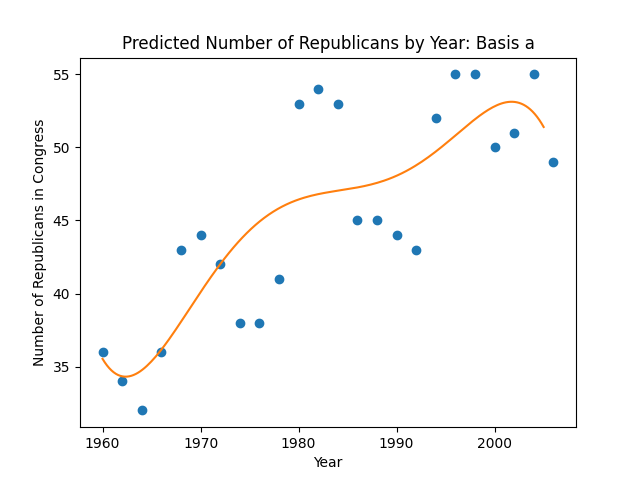
\includegraphics[scale=0.75]{yeara.png} \\

\textbf{$\mcL(w^*) = 197.4902$} \\

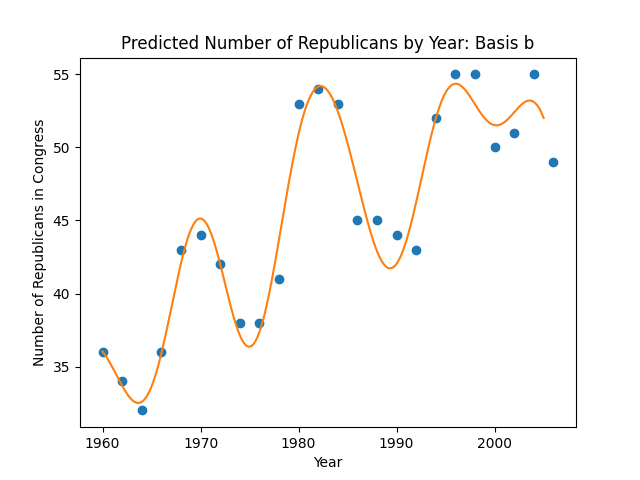
\includegraphics[scale=0.75]{yearb.png}\\

\textbf{$\mcL(w^*) = 27.1365$} \\

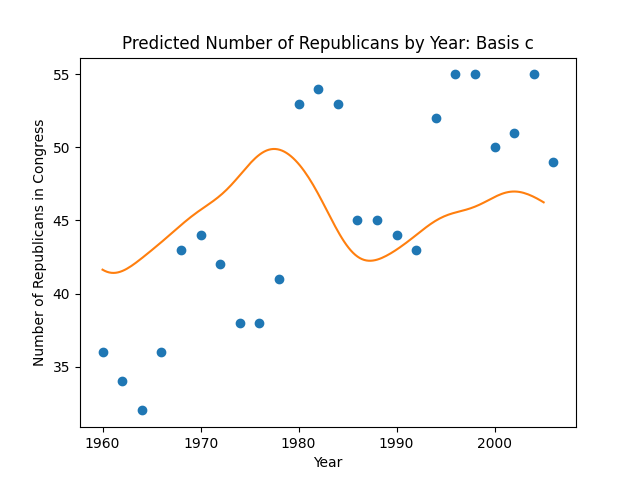
\includegraphics[scale=0.75]{yearc.png}\\

\textbf{$\mcL(w^*) = 541.4044$} \\

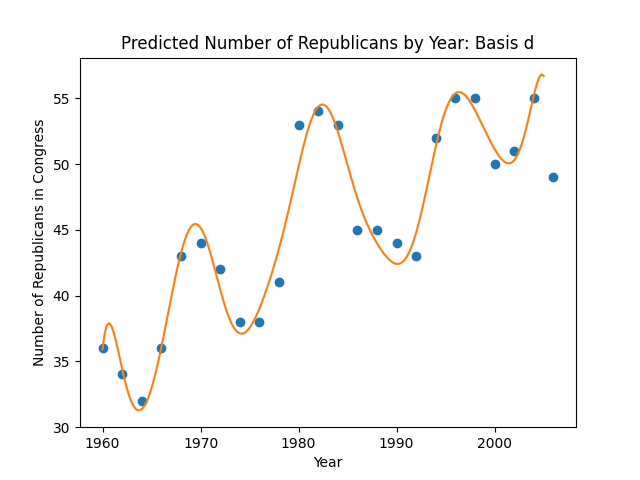
\includegraphics[scale=0.75]{yeard.png}\\

\textbf{$\mcL(w^*) = 19.5006$} \\

\newpage

\noin \textbf{Solution 4.2}

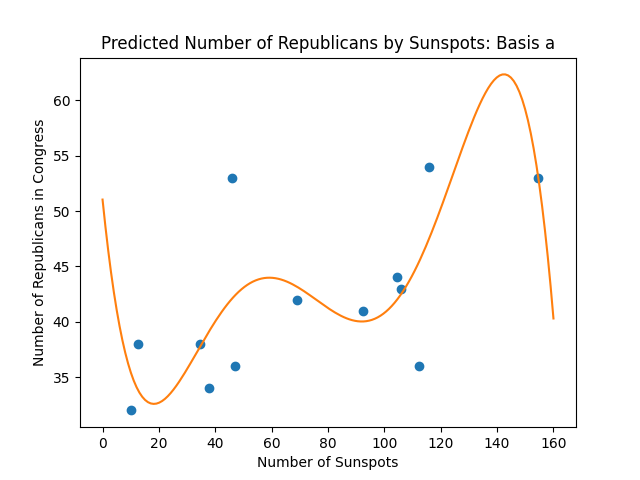
\includegraphics[scale=0.75]{sunspota.png} \\

\textbf{$\mcL(w^*) = 175.6139$} \\

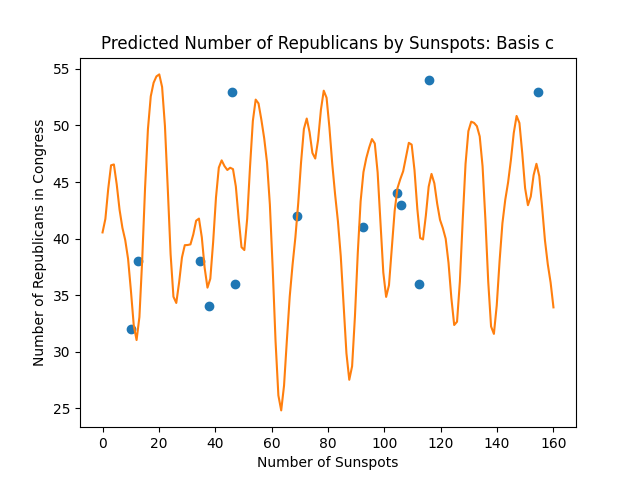
\includegraphics[scale=0.75]{sunspotc.png}\\

\textbf{$\mcL(w^*) = 187.5534$} \\

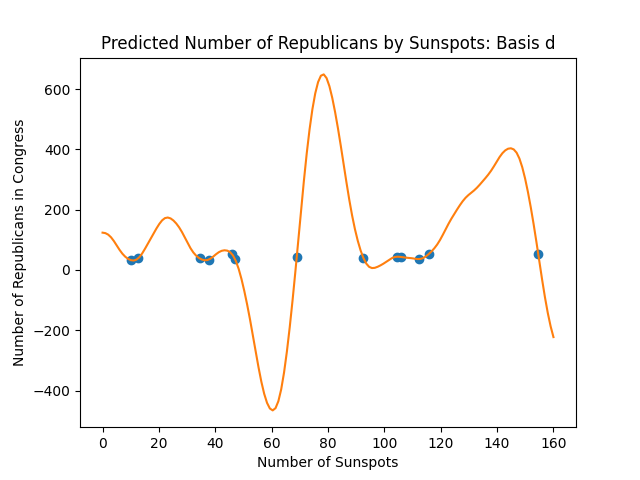
\includegraphics[scale=0.75]{sunspotd.png}\\

\textbf{$\mcL(w^*) = 4.3049$} \\ \\
Of the three bases, basis (a) provided the "best" fit. Looking at basis (d), while there is very little loss, the model predicts negative numbers of republicans in Congress, which is quite obviously impossible. As such, the model has very poor generalizability despite its high accuracy on the training data and thus is not a good fit. Looking at basis (c), we see that the model fluctuates wildy between small increments along the $x$ axis. From a rational standpoint, it is very unlikely that the relationship between sunspots and republicans fluctuates dramatically as shown in this model, so it too has poor generalizability. Moreover, this model has the highest loss. Comparatively, basis (a) has a fairly steady curve and does not fluctuate wildly like basis (c). Additionally, it has slightly lower loss than basis (c). As such, it provides the "best" fit of the three bases. \\ \\
Given the quality of this fit, I do not believe that the number of sunspots controls the number of Republicans in the senate. Our choice of basis (a) as the "best" fit was really a choice of the best of three bad options. Of the two models not chosen, one made impossible predictions while the other was modeled after a bizarre and dramatically fluctuating function. Even with these poor options, this basis only performed slightly better in terms of loss and when looking at the graph, the function only appears to loosely fit the training data set. Moreover, taking a step back, rationally, it is extremely unlikely that something completely unrelated like the number of sunspots observed bears any meaningful effect on the number of republicans in congress.



\newpage
%%%%%%%%%%%%%%%%%%%%%%%%%%%%%%%%%%%%%%%%%%%%%
% Name and Calibration
%%%%%%%%%%%%%%%%%%%%%%%%%%%%%%%%%%%%%%%%%%%%%
\subsection*{Name:}
\\ \\ 
Jamin Liu

\subsection*{Collaborators and Resources}
Whom did you work with, and did you use any resources beyond cs181-textbook and your notes? \\ \\
N/A

\subsection*{Calibration}
Approximately how long did this homework take you to complete (in hours)? 
\\\\ 8 hours
\end{document}